\chapter{Coloured de Bruijn Graphs}
%Now consider a de Bruijn graph for a large population of samples, whereby we want to accurately recover the
%sample set ids from a given node or edge.
%Hospitals sequencing to test for genes (instead of genotyping) as cost is decreasing

\section{Adding Color}
\label{subsec:color}

Given a multiset \(\mathcal{G} = \{G_1, \ldots, G_t\}\) of individual de Bruijn graphs, we set $G$ to be the union of those individual graphs and build the BOSS representation for $G$.  We also build and store a two-dimensional binary array $C$ in which \(C [i, j]\) indicates whether the $i$th edge in $G$ is present in the $j$th individual de Bruijn graph (i.e., whether that edge has the $j$th color). 
(Recall from the description above that we consider the edges in $G$ to be sorted lexicographically by the reversed labels of their starting nodes, with ties broken lexicographically by their own single-character labels.)  
%(For technical reasons that are explained below, we consider the edges in $G$ to be sorted lexicographically by the reversed labels of their starting nodes, with ties broken lexicographically by their own (single-character) labels.)  
We keep $C$ compressed, but in such a way that we can still access individual bits quickly.  If the individual graphs are similar, then most edges will appear in most graphs, so it is more natural to use 0s to indicate that edges are present and 1s to indicate that they are absent.  With these data structures, we can navigate efficiently in any of the individual graphs.

%Figure~\ref{fig:purple} shows an example of how we represent a colored de Bruijn graph consisting of two individual de Bruijn graphs.  Suppose we are at node {\tt ACG} in the graph, which is the co-lexicographically eighth node.  Since the eighth 1 in $B_L$ is \(B_L [10]\) and it is preceded by two 0s, we see that {\tt ACG}'s outgoing edges' labels are in \(\EBWT [8..10]\), so they are {\tt A}, {\tt C} and {\tt T}.  Suppose we want to follow the outgoing edge $e$ labelled {\tt C}.  We see from \(C [9, 0..1]\) (i.e., the tenth column in $C^\mathrm{T}$) that $e$ appears in the second individual graph but not the first one (i.e., it is blue but not red).    There are four edges labelled {\tt A} in the graph and three {\tt C}s in \(\EBWT (G) [0..9]\), so $e$ is \(F [6]\).  (Since edges labelled {\tt \$} have only one end, they are not included in $L$ or $F$.)  From counting the 1s in \(B_F [0..6]\), we see that $e$ arrives at the fifth node in co-lexicographic order that has incoming edges.  Since the first node, {\tt \$\$\$}, has no incoming edges, that means $e$ arrives at the sixth node in co-lexicographic order, {\tt CGC}.

\begin{landscape}
\begin{figure*}
\begin{tabular}{c@{\hspace{0.03\textwidth}}c@{\hspace{0.03\textwidth}}c}
%\includegraphics[width=.31\textwidth]{images/greyscale_purplegraph.eps} &
\includegraphics[width=.31\textwidth]{greyscale_purplegraph} &
%\includegraphics[width=.31\textwidth]{images/greyscale_newpurplemapping.eps} &
\includegraphics[width=.31\textwidth]{greyscale_newpurplemapping} &
\raisebox{9ex}{$\begin{array}{rr}
   \EBWT (G) = \hspace{-7.5ex} &\\[1ex]
               & \mathtt{TCCGTGGGACTAAA\$C}\\[1ex]
         B_F = & \mathtt{ 001111110111111}\\
         B_L = & \mathtt{1110111100111111}\\[1ex]
C^\mathrm{T} = & \mathtt{0000001001010000}\\
               & \mathtt{0000000110101001}
\end{array}$}
\end{tabular}
\caption{{\bf Left:} A colored de Bruijn graph consisting of two individual graphs, whose edges are shown in light gray and black.  (We can consider all nodes to be present in both graphs, so they are shown in dark gray.)  {\bf Center:} The nodes sorted into co-lexicographic order, with each node's number of incoming edges shown on its left and the labels of its outgoing edges shown on its right.  The edge labels are shown in light gray or black if the edges occur only in the respective graph, or dark gray  if they occur in both.  {\bf Right:} Our representation of the colored de Bruijn graph: the edge-BWT and bitvectors for the BOSS representation for the union of the individual graphs, and the binary array $C$ (shown transposed) whose bits indicate which edges are present in which individual graphs.}
\label{fig:purple}
\end{figure*}
\end{landscape}

\section{Implementation}
\label{subsec:implementation}

We now give some details of how our data structure is implemented and constructed in practice.

\subsection{Data Structure}

The arsenal of component tools available to succinct data structures designers has grown considerably in recent years, with many methods now implemented in libraries. We chose to make heavy use of the succinct data structures library (SDSL)\footnote{\url{https://github.com/simongog/sdsl-lite}} 
in our implementation.

\(\EBWT (G)\), the sequence of edge labels, is encoded in a wavelet tree, which allows us to perform fast rank queries, essential to all our graph navigations. The bitvectors of the wavelet tree  and the $B$ bitvector are stored in the RRR encoding
%[SJP: RRR will be significantly slower than a plain encoding, and I'm not sure it will reduce the size of the WT very much - this is something we need to test. We might even want to use something other than a WT].
The rows of the color matrix, $C$, are concatenated (i.e. $C$ is stored in row-major order) and this single long bit string is then compressed.  It is either stored with RRR encoding,  or alternately Elias-Fano encoding which supports online construction.  Online construction is important for datasets where $C$ is too large to fit in memory in uncompressed form, such as our metagenomic sample dataset.  These encodings reduce the size of $C$ considerably because we expect rows to be very sparse
%(i.e. most $k$-mers are contained in most samples),
and both encodings exploit this sparseness. 
%[SJP: we really should be using the access-optimised encoding that Travis and I suggested --- RRR is overkill and likely slower].

\subsection{Construction}


In order to convert the input data to the format required by BOSS (that is, in correct sorted order, including dummy edges and bit vectors), we use the following process.  We take care to ensure only subsets of data are needed in RAM at any one time during construction.

%First, 
%we read the header of the Cortex graph format, then iterate over the $(k-1)$-mers. For each $(k-1)$-mer, Cortex provides a bit matrix, where each row is a colour, and each
%column is a flag to indicate outgoing edges present in that colour. We invert this matrix to give us a bitmap representing the colours that each outgoing edge symbol is a member of.

Our construction algorithm takes as input the set of ($k$-mer, color-set) pairs present in the input sets of reads, or alternately, $k$-mer counts for each color which we convert to the former ourselves.
Here, color-set is a bit set indicating which samples the $k$-mer occurs in.
We provide the option to use the {\sc Cortex} frontend to generate the ($k$-mer, color-set). Unfortunately, this also limits the datasets to those that would run through {\sc Cortex}.  To overcome this, we provide the option to use a list of KMC2~\citep{KMC2} sorted $k$-mer counts as input.  With this option, the $k$-mers from each $k$-mer count file in native KMC2 binary format are streamed through a priority queue to produce the union of all $k$-mer sets; initially one $k$-mer from each file is tagged with  which file it originated from, and the ($k$-mer, file ID) pair is added to the queue.   The priority queue ensures the lexicographically smallest $k$-mer instances across all files can be popped off the queue consecutively.  All of the $k$-mer count files contributing a particular $k$-mer value have their corresponding color recorded as `1' bits in the bit set for that $k$-mer.  Both the $k$-mer and the bit set are then appended to vectors which optionally are allocated in external memory using the STXXL\footnote{\url{http://stxxl.sourceforge.net/}} library.   As each $k$-mer is popped off the queue, another $k$-mer is added to the queue to take the old $k$-mer's place (i.e. using the file identified by the popped $k$-mer's tag).  This process continues until all files are read in their entirety.  By both streaming data from the source files and streaming it to the external vectors, only a small amount of the data need exist in memory at a time; the priority queue will only contain the number of samples and only one row of the color matrix needs to exist in memory before being written out to disk.

%This effectively gives us ($k$-mer, color-set) pairs\footnote{In our current implementation, the color-set bitmaps were chosen to be 64 bits wide for simplicity, but can easily be extended to wider
%(or variable-length) bitmaps.}.

After constructing the initial union set of $k$-mers and their corresponding color rows, BOSS construction mostly continues as originally described by Bowe {\it et al.}.  The changes from the original construction algorithm are that most of the data optionally resides in external memory and the rows of the color matrix are permuted with their corresponding $k$-mers as they are sorted.  For each of the $k$-mers we generate the reverse complement (giving it the same color-set as its twin). Then, for each $k$-mer (including the reverse complements),
we sort the ($k$-mer, color-set) pairs by the first $k-1$ symbols (the source node of the edge) to give the $F$ table (from here, the colors are moved around with rows of $F$, but otherwise ignored until 
the final stage). Independently, we sort the $k$-mers (without the color-sets) by the last $k-1$ symbols (the destination node of the edge) to give the $L$ table.

With $F$ and $L$ tables computed, we calculate the set difference $F-L$ (comparing only the $(k-1)$-length prefixes and suffixes respectively), which tells us which nodes require incoming dummy edges. Each such node is then
shifted and prepended with $\$$ signs to create the required incoming dummy edges ($k-1$ each). These incoming dummy edges are then sorted by the first $k-1$ symbols.
Let this table of sorted dummy edges be $D$. Note that the set difference $L - F$ will give the nodes requiring outgoing dummy edges, but these do not require sorting, and so we can calculate it as is needed in the final stage.

Finally, we perform a three-way merge (by first $k-1$ symbols) $D$ with $F$, and $L-F$ (calculated on the fly). For each resulting edge, we keep track of runs of equal $k-1$ length prefixes,
and $k-2$ length suffixes of the source node, which allows us to calculate the $B_F$ and $B_L$ bit vectors, respectively. Next, we write the bit vectors, symbols from last column, and
count of the second to last column to a packed file on disk, and the colors to a separate file.   The color file is then either buffered in RAM and RRR encoded or optionally streamed from disk and then Elias-Fano encoded online (i.e. only the compressed version is ever resident).  The time bottleneck in the above process is clearly in sorting the $D$ and $F$ tables, which are of the same size, and are made up of elements of size $O(k)$. Thus, overall, construction of the data structure takes $O(k(|F|\log|F|))$ time.



%TODO: Asymptotics? We should also say that we use STXXL (which will give us EM sorting bounds)
% Reading: O(N) (# nodes) x O(sigma|C|)
% Sorting: O(|F| log |F|)
% F-L: O(|F|)
% Sort dummies: O(|D| log |D|)
% Final Merge: O(|F| + |D|) (|D| <= |F| -> O(|F|))

%[SJP: The following overly detailed description is from Alex. To be refined.]
%
%Getting + sorting necessary kmers
%1 read in the node, coverages and edge bitmaps
%2 iterate over the color bitmap, then in an inner loop iterate over
%edge symbols. I then make an inverted symbol by color bit matrix
%3 for each symbol that has a non-zerod row in the matrix, I shift the
%node and append the symbol to make a k-mer (edge)
%4 I reverse the nucleotides of the kmer so it will be sorted in colex
%order, and I also compute the reverse complement
%5 I add (kmer, color-bitmap), (revcomp, color-bitmap) pairs to a
%sorting container (which generates runs, then merges them on access
%later) which drops the last symbol before sorting (table F)
%6 I also add the kmer and revcomp (no color data) to another sorting
%container which sorts based on the whole string (table L)
%Note: In the old version, only 6 was done. The radix sort used two
%tables, so by saving the buffer table we had the second-last iteration
%as well, which meant we had table F
%Note: 5 and 6 are sorted in parallel on different disks for my
%version, so it is faster than a multi-pass version (tested), but also
%uses 2x the disk space. It isnt a radix sort though, so it doesnt
%double the table size. i.e. for both implementations, we use 2x the number 
%of input kmers to add rev comps, then 2x again for F and L.
%
%Generating incoming dummy edges:
%7. i use std::set-difference to take both tables (wrapping the
%iterator so access return just the first k-1 syms from kmers in of F,
%and the last k-1 syms from kmers in L, and both made to be unique - no
%duplicates). This calculates F - L, since any node without a
%predecessor needs an incoming dummy.
%8. it outputs the k-1-mers from F to a provided function, which loops
%(k-2) times to generate \$... \$\$... \$\$\$... (these extra shifts aren't
%technically needed, except to be able to generate the labels for
%incoming dummies again)
%9. each of these is added to another sorter, like above, to be sorted
%on their first k-1 symbols (with \$ sorting before any other symbols).
%Note: before 9, even without all the shifts, the dummies are output in
%the same order as L (colex of whole edge).
%Note: colors dont need to be looked at here (we treat dummies as
%having 0 color for now)
%
%Merging and outgoing dummies:
%Note: You could do a L-F set difference to get outgoing dummies, but
%they are generated in the right order for F, so I combined them into
%one big merge step at the end.
%10. I make a wrapped iterator to access F without the color
%information, but to save it to a color variable that is in scope. This
%way I can merge the color in as I'm writing the kmers out.
%11. I take the two tables F and L, and the dummies. I merge the
%dummies into F (although this time comparing all k symbols), but I
%also calculate the L-F set difference as I'm going. Kind of like a
%3-way merge. If a node is in L that isnt in F, I shift that node and
%append a $ on the right: ....$
%12. each of these is sent to a function, which checks all the first
%k-1 symbols, and last k-1 symbols to generate the B and B' vectors
%(which show the range of entries for nodes in L and F)
%13. the last symbol is written to a file along with the bit vectors
%(interleaved and packed into 64bit blocks)
%14. the color (which is a variable that is now overwritten by the
%iterator wrapper) is written to a separate file.
%
%
%\begin{figure}
%\begin{center}
%\includegraphics[width=.5\textwidth]{New+Doc+5_1.jpg} \\[10ex]
%\caption{Construction of the succinct colored de Bruijn graph, from input to output.}
%\label{fig:construction}
%\end{center}
%\end{figure}

\subsubsection{Traversal}
We implemented three traversal methods based on those of {\sc Cortex} and the intention to apply $\ours$ to metagenomic reads and look for AMR gene presence.

The first, {\it bubble calling}, is a simple algorithm to detect sequence variation in genomic data. It consists of iterating over a set of $k$-mers in order to find places where bubbles start and terminate.  When combined with the $k$-mer color (in a colored de Bruijn graph), this enables identification of places where genomic sequences diverge from one another.  The differing region of the two sequence will form the two arms of a bubble, each colored with only one of the two sequence's colors.  A bubble is identified when a vertex has two outgoing edges. Each edge is followed in turn to navigate a non-branching path until reaching a vertex with two incoming edges. If the terminating vertex is the same for both paths, we call this a bubble. Colors for the bubbles are determined by looking at the color assignment of the corresponding $(k)$-mers. Our implementation in $\ours$ closely follows the pseudocode given by \cite{ICTFM12}; however, it navigates the graph only in a forward direction to see if both paths converge at the same vertex, while {\sc Cortex} navigates the graph backwards and forwards to find a path of adjacent vertices.

For metagenomic experiments, we count the number of $k$-mers in common between the metagenomic sample and each of the AMR genes.  If each AMR gene is available as a separate color, the set operations can be done with a linear traversal of the intermediate file containing the uncompressed $C$ matrix.  In this case, loading and traversing the colored de Bruijn graph is not necessary.  We refer to this matrix scan algorithm as {\it match color}. 

For the beef safety experiments, we implemented an algorithm derived from {\sc Cortex}'s {\it path divergence} algorithm.  In the {\sc Cortex} path divergence algorithm, bubbles are identified where a reference sequence may walk a tangled sections of the graph in its arm of the bubble while the alternative arm must be branch free.  Because we have the reference to guide the traversal, all AMR genes can be combined into a single color.  By combining AMR genes, the uncompressed color matrix that exists on disk during sorting is much smaller, thus accelerating the permutation during construction and reducing the external memory and disk space requirements.

As we are interested specifically in the presence of AMR genes (our reference sequence), in our derived algorithm we ignore sample path segments leading away from and returning to the AMR gene path; As we traverse the gene path, we simply count the number of samples in each sample group that color the current edge.   We note that keeping $C$ in row major order allows us to compute this count in constant time as the difference between two $\rank$ queries.


%\section{Cortex Algorithms}
